\title{\textbf{Half of All Liquidations Are Unseen at the Close}\\[0.3em]
\large Path Risk versus Close-to-Close Volatility in Crypto Perpetual Futures\iftechnical\else\\[0.2em]
\normalsize Reader edition\fi}
\author{Ricardo P\'erez Twerdy\thanks{Contact: \href{mailto:rtwerdy@gmail.com}{rtwerdy@gmail.com}.
This paper is independent research. It is not affiliated with, sponsored by, or related in any way
to the author's work at Coinbase, and it does not represent the views of Coinbase. Nothing in it is
investment advice.\iftechnical\ A reader edition without the stochastic framework is available in
the repository cited in Section~\ref{sec:conclusion}.\else\ The technical edition, with the full
stochastic framework, is available in the repository cited in Section~\ref{sec:conclusion}.\fi}}
\date{November 2026}

\begin{document}
\maketitle

\begin{abstract}
\noindent
\iftechnical
Risk measures for leveraged positions are routinely estimated from close-to-close returns, while
liquidation engines in crypto perpetual futures monitor the mark price continuously and liquidate at
the first touch of the liquidation boundary. We formalise the gap as the difference between a
first-passage event and a terminal event, and derive its Brownian benchmarks: half of all boundary
crossings are invisible at the end of the horizon, and the 99th-percentile path loss exceeds the
terminal loss by a factor of $1.107$.
\else
Most risk measures in crypto, volatility and value-at-risk among them, are computed from closing
prices. Liquidation engines do not wait for the
close: they watch the mark price continuously and close a leveraged position the moment it touches
its liquidation level. Even in an idealised random market, a view based on closing prices misses
half of those liquidations, and understates the 1-in-100 adverse move by about 11\%.
\fi
We measure both effects on 12 months of 1-minute mark prices for every USDT-margined perpetual
listed on Binance, delisted contracts included, using each contract's own maintenance-margin rate
and maximum leverage. Higher leverage brings more liquidations, not a smaller blind spot. Outside
BTC and ETH, a long held for a day in a smaller contract (our Tail tier) is liquidated in \TailDayLongPP{} of windows at 10x
and in \TailDayLongPPTwentyFive{} at 25x, the median leverage on offer at Binance and Bybit, while
only \TailDayLongPC{} and \TailDayLongPCTwentyFive{} end beyond the liquidation level. The share of
liquidations that the close misses stays near one half at every leverage: \UTenLo--\UTenHi\% at
10x and \UTwentyFiveLo--\UTwentyFiveHi\% at 25x. The 99th-percentile adverse move along the path is
\KappaLo{} to \KappaHi{} times the 99th-percentile close-to-close loss, against $1.107$ for a random
walk, and is largest for short positions in newly listed contracts. The results hold on a balanced
cohort of surviving contracts.
\end{abstract}

\section{Introduction}

Most risk measures, volatility and value-at-risk among them, are still computed as in equity
markets: one price per period, the close, and returns between closes. Leveraged positions in crypto
perpetual futures do not live on closes; they live on the path. The exchange's liquidation engine
watches the mark price continuously and closes a position the moment it touches the liquidation
level. Crypto perpetuals differ from a closing-price world in three ways:
\begin{itemize}\itemsep0pt
\item the market never closes, so a daily ``close'' is an arbitrary timestamp;
\item liquidation engines monitor the mark price continuously and act within seconds;
\item a position liquidated at 03:00 stays liquidated, whatever the price does by midnight.
\end{itemize}
This paper measures how large the resulting blind spot is, across the whole Binance perpetual
market and over a full year.

\paragraph{Leverage.} The blind spot matters because of the leverage on offer
(Table~\ref{tab:venues}). Binance and Bybit allow up to 150x on their BTC and ETH perpetuals, OKX up
to 100x, Deribit up to 50x on its linear USDC perpetuals, and Hyperliquid up to 40x. Smaller
contracts offer less, but not little: the median contract allows 25x on Binance and Bybit and 20x on
OKX, and between 17\% and 37\% of contracts on these three venues allow 50x or more. The liquidation
level sits at $1/L$ minus the maintenance-margin rate (Section~\ref{sec:liq}). For BTC on Binance, with a
maintenance-margin rate of 0.4\%, a long is liquidated after a fall of 9.6\% at 10x, 3.6\% at 25x and
1.6\% at 50x. Liquid crypto assets make such moves within hours, often within minutes. Binance,
Bybit, OKX and Hyperliquid all document that liquidation is triggered by a mark price rather than by
the last traded price~\cite{binance-liq,bybit-mark,okx-liq,hl-liq}, so the analysis uses Binance's
mark price throughout.

\begin{table}[t]
\centering
\caption{Maximum leverage on linear (USDT- or USDC-margined) perpetuals, retrieved from each venue's
public market-data interface on 22 November 2026. \emph{BTC}: the venue's linear BTC perpetual.
\emph{Median}, $\geq$\,50x, $\leq$\,10x: across all listed contracts. Binance values are for the
first (smallest-notional) risk bracket. Sources:
\cite{binance-brackets,bybit-api,okx-api,deribit-api,hl-api}.}
\label{tab:venues}
\small
\begin{tabular}{@{}lrrrrrr@{}}
\toprule
Venue & Contracts & BTC & Highest & Median & $\geq$ 50x & $\leq$ 10x \\
\midrule
Binance & 930 & 150x & 150x & 25x & 37\% & 22\% \\
Bybit & 831 & 150x & 150x & 25x & 23\% & 5\% \\
OKX & 531 & 100x & 100x & 20x & 17\% & 28\% \\
Deribit & 152 & 50x & 50x & 10x & 14\% & 55\% \\
Hyperliquid & 179 & 40x & 40x & 5x & 0\% & 98\% \\
\bottomrule
\end{tabular}

\end{table}

\paragraph{An example.} Figure~\ref{fig:example} shows one 24-hour window on BTCUSDT, the most
liquid perpetual in the market. A long position opened at 17:00 UTC on 5 February 2026 ended the
window \textbf{2.4\% above entry}. A risk model built on closing prices records a profitable,
unremarkable day. Along the way, the mark price fell 12.1\% below entry. A 50x long was liquidated
after \EXFIFTY{} hours (twelve minutes), a 25x long after \EXTWENTYFIVE{} hours, and a 10x long after
\EXTEN{} hours.

\begin{figure}[t]
\centering
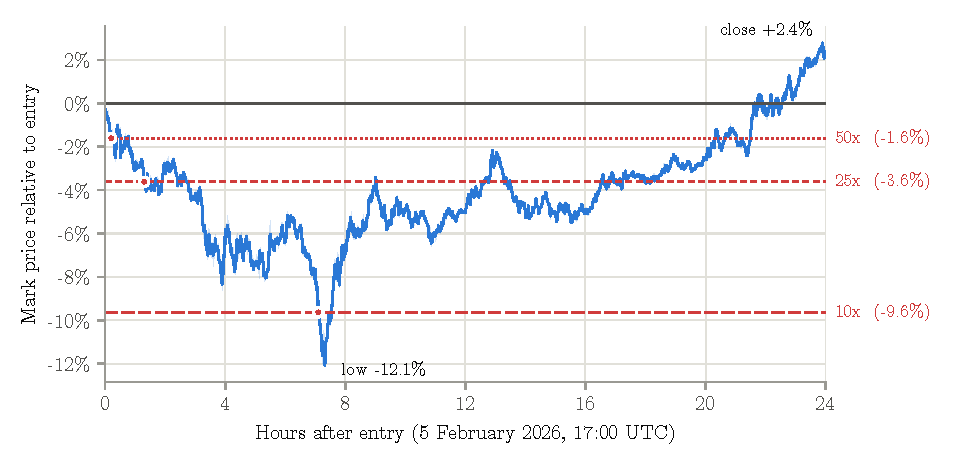
\includegraphics[width=\linewidth]{figures/fig1_example.pdf}
\caption{BTCUSDT mark price relative to entry, 24 hours from 5 February 2026 17:00 UTC. The shaded
band is each minute's high--low range. Dashed lines: liquidation levels of isolated longs at 10x,
25x and 50x, which with BTCUSDT's 0.4\% maintenance-margin rate sit at $-9.6\%$, $-3.6\%$ and
$-1.6\%$ (Section~\ref{sec:liq}); dots mark the first touch of each. A close-to-close view sees
$+2.4\%$.}
\label{fig:example}
\end{figure}

\paragraph{What we do.} \iftechnical We formalise liquidation as a first-passage event and the
close-to-close view as a terminal event, and derive their Brownian benchmarks
(Section~\ref{sec:framework}).\else We explain why a view based on closing prices misses about half
of all liquidations even in an idealised market (Section~\ref{sec:framework}).\fi{} We build a
point-in-time, survivorship-free universe of 753 Binance perpetuals over 12 months
(Section~\ref{sec:data}). We then measure, across liquidity tiers, horizons, sides and leverage
levels, how often liquidations are unseen at the close and how much heavier the tail of the path is
than the tail of the close (Sections~\ref{sec:results} and~\ref{sec:robust}).

\iftechnical
\section{Stochastic framework}
\label{sec:framework}

\subsection{Setting}

Let $(\Omega,\F,\mathbb{F},\Prob)$ be a filtered probability space, with filtration
$\mathbb{F}=(\F_t)_{t\ge 0}$ satisfying the usual conditions. The mark price $(M_t)_{t\ge0}$ of a
perpetual contract is a strictly positive, $\mathbb{F}$-adapted process with c\`adl\`ag paths. A
position opened at time $t_0$ and held for a horizon $h>0$ has log-return process
\begin{equation}
X_t = \log\frac{M_{t_0+t}}{M_{t_0}}, \qquad 0\le t\le h,
\end{equation}
with running minimum and maximum $\underline{X}_h=\inf_{0\le t\le h}X_t$ and
$\overline{X}_h=\sup_{0\le t\le h}X_t$.

A long position is liquidated when the mark price falls by a fraction $d_\ell\in(0,1)$ from entry,
and a short when it rises by $d_s>0$ (Section~\ref{sec:liq} derives $d_\ell$ and $d_s$). In log terms
the boundaries are $b_\ell=-\log(1-d_\ell)$ and $b_s=\log(1+d_s)$.

\begin{definition}[Liquidation time]
The liquidation time of a long position is the first-passage time
\begin{equation}
\tau_\ell=\inf\{t\in[0,h]: X_t\le -b_\ell\}, \qquad \inf\emptyset=+\infty,
\end{equation}
and analogously $\tau_s=\inf\{t\in[0,h]:X_t\ge b_s\}$ for a short. Since $X$ is c\`adl\`ag and
adapted and $\mathbb{F}$ satisfies the usual conditions, $\tau_\ell$ and $\tau_s$ are stopping times
(the d\'ebut theorem).
\end{definition}

\begin{definition}[Path and close breaches]
For a long position, the \emph{path breach} is the event $A_P=\{\tau_\ell\le h\}=\{\underline{X}_h\le
-b_\ell\}$ and the \emph{close breach} is the event $A_C=\{X_h\le -b_\ell\}$, with probabilities
$p_P=\Prob(A_P)$ and $p_C=\Prob(A_C)$. Since $X_h\ge\underline{X}_h$, $A_C\subseteq A_P$. The
\emph{unseen share} is the fraction of liquidations that a close-to-close observer does not record:
\begin{equation}
U=\Prob\big(A_C^{c}\,\big|\,A_P\big)=1-\frac{p_C}{p_P}.
\end{equation}
For a level $\alpha\in(\tfrac12,1)$, the \emph{path-to-close quantile multiple} is
\begin{equation}
\kappa_\alpha=\frac{Q_\alpha\big(-\underline{X}_h\big)}{Q_\alpha\big(-X_h\big)},
\end{equation}
where $Q_\alpha$ denotes the $\alpha$-quantile. Short positions use $\overline{X}_h$, $X_h$ and
$b_s$ symmetrically.
\end{definition}

$U$ measures how often a close-to-close view misses a liquidation; $\kappa_\alpha$ measures by how
much it understates the tail of the adverse move. Neither requires a model of $M$, and both have
exact benchmarks under Brownian motion.

\subsection{The Brownian benchmark}

Suppose $X_t=\sigma W_t$, with $W$ a standard $\mathbb{F}$-Brownian motion and $\sigma>0$.

\begin{proposition}[Reflection principle]
\label{prop:reflection}
For every $b>0$,
\begin{equation}
\Prob\big(\underline{X}_h\le -b\big)=2\,\Prob\big(X_h\le -b\big)=2\,\Phi\!\left(-\frac{b}{\sigma\sqrt h}\right),
\end{equation}
where $\Phi$ is the standard normal distribution function.
\end{proposition}

\begin{proof}[Sketch]
Let $\tau=\inf\{t:W_t=-b/\sigma\}$. On $\{\tau\le h\}$, the strong Markov property and the symmetry
of Brownian increments give $\Prob(W_h\le -b/\sigma\mid\F_\tau)=\tfrac12$. Since $\{X_h\le
-b\}\subseteq\{\tau\le h\}$, it follows that $\Prob(X_h\le-b)=\tfrac12\Prob(\tau\le h)$.
\end{proof}

\begin{corollary}
\label{cor:half}
Under Brownian motion, $U=\tfrac12$ for every boundary $b$, volatility $\sigma$ and horizon $h$:
half of all liquidations are invisible at the close, whatever the leverage.
\end{corollary}

\begin{proposition}[Quantile multiple]
\label{prop:kappa}
Under Brownian motion, $\kappa_\alpha=z_{(1+\alpha)/2}/z_\alpha$, where $z_p=\Phi^{-1}(p)$. In
particular, $\kappa_{0.99}=2.5758/2.3263=1.107$.
\end{proposition}

\begin{proof}
By Proposition~\ref{prop:reflection}, $\Prob(-\underline{X}_h>x)=2\Phi(-x/(\sigma\sqrt h))$ for
$x>0$. Setting this equal to $1-\alpha$ gives $Q_\alpha(-\underline{X}_h)=\sigma\sqrt h\,
z_{(1+\alpha)/2}$, while $Q_\alpha(-X_h)=\sigma\sqrt h\,z_\alpha$.
\end{proof}

\begin{remark}[Drift]
With drift, $X_t=\mu t+\sigma W_t$, the first-passage probability becomes
$\Phi\big(\tfrac{-b-\mu h}{\sigma\sqrt h}\big)+e^{-2\mu b/\sigma^2}\Phi\big(\tfrac{-b+\mu h}{\sigma\sqrt h}\big)$.
Over horizons of hours to a day, $\mu h$ is negligible relative to $\sigma\sqrt h$, and the
benchmarks above are unchanged to the precision reported here.
\end{remark}

\begin{remark}[Discrete monitoring]
If the path were observed only at times $k\Delta$, the observed minimum would exceed
$\underline{X}_h$ and touches between observations would be missed. Broadie, Glasserman and
Kou~\cite{bgk} show that discrete monitoring is equivalent, to first order, to shifting the boundary
outward by $\beta\sigma\sqrt\Delta$, with $\beta=-\zeta(\tfrac12)/\sqrt{2\pi}\approx0.5826$, which
lowers $U$ below $\tfrac12$. Our data record the highest and lowest mark price within each minute, so
the path is observed at the frequency at which the venue updates its mark price (a few seconds). The
effective $\Delta$ is small and the Brownian benchmark is close to $\tfrac12$.
\end{remark}

\subsection{Departures from the benchmark}

Real mark-price paths are not Brownian. Heavy-tailed returns, jumps, and transient dislocations that
revert (``wicks'', often caused by forced liquidations themselves) make the running extremum heavier
relative to the terminal value. They raise $\kappa_\alpha$ above $1.107$ and, when the dislocation
reverts within the horizon, raise $U$ above $\tfrac12$. Persistent trends act in the opposite
direction on $U$. The two statistics are therefore model-free diagnostics: $U$ measures \emph{how
often} the close misses the liquidation, and $\kappa_\alpha$ measures \emph{how far} the close
understates the adverse tail, each against an exact benchmark. Range-based volatility
estimators~\cite{parkinson,garmanklass,rogerssatchell} rest on the same observation: the extremes of
a path carry information that the close discards.
\else
\section{Why the close misses half of all liquidations}
\label{sec:framework}

Take a position with a liquidation level some distance below its entry price, and compare two
questions over the same holding period:
\begin{itemize}\itemsep0pt
\item \emph{close view}: does the price \emph{end} the period below the liquidation level?
\item \emph{path view}: does the price \emph{touch} the liquidation level at any time during the
period? This is what the liquidation engine checks.
\end{itemize}
Every close breach is also a path breach, but not the reverse: a price can dip through the level and
recover before the period ends. We call the fraction of liquidations that the close view misses the
\textbf{unseen share}, $U$.

\paragraph{The random-walk benchmark.} Suppose prices followed a pure random walk, with no trend and
no fat tails. Consider any path that touches the liquidation level. From that moment on, the walk is
as likely to go up as down, so it is as likely to end above the level as below it. Half of the paths
that touch the level therefore end above it, and the close view never records them: $U=50\%$. This is
the \emph{reflection principle}, and it holds for every volatility, horizon and leverage. Even in the
gentlest possible market, a risk measure built on closing prices misses half of all liquidations.

The same argument applies to tail risk. In a random walk, the 1-in-100 worst move \emph{along the
path} is $1.107$ times the 1-in-100 worst move \emph{at the close}: closing prices understate the
1-in-100 adverse move by about 11\%. We call this ratio the \textbf{quantile multiple}, $\kappa$.

\paragraph{What real prices add.} Crypto prices are not a random walk. Fat tails, jumps, and sharp
spikes that reverse (``wicks'', often caused by forced liquidations themselves) make the worst point
of a path more extreme relative to where the path ends. They push $\kappa$ above $1.107$ and, when the
spike reverses within the holding period, push $U$ above 50\%. Both measures can therefore be read
against a clean benchmark: $U$ against 50\%, $\kappa$ against $1.107$. Volatility estimators that use
highs and lows, not only closes~\cite{parkinson,garmanklass,rogerssatchell}, rest on the same idea.

One technical point: the benchmark assumes the liquidation level is checked continuously. Our data
record the highest and lowest mark price within each minute, so the path is effectively checked at
the venue's mark-price update frequency, every few seconds, and the 50\% benchmark applies.
\fi

\section{Data and a point-in-time universe}
\label{sec:data}

\paragraph{Prices.} We use Binance USDT-margined perpetual futures from the public archive at
\url{https://data.binance.vision}: 1-minute mark-price candles, the price on which Binance triggers
liquidation~\cite{binance-liq}, and, for robustness, 1-minute last-traded-price candles. The archive
retains files for delisted contracts, so the sample is free of survivorship bias at the source.

\paragraph{A universe that changes.} The set of tradable perpetuals in October 2026 differs from the
set in November 2025: \ListingsN{} contracts were listed during the period and \DelistingsN{} were
delisted.\footnote{On average \ListingsPerMonth{} listings and \DelistingsPerMonth{} delistings per
month between November 2025 and October 2026, with monthly listings ranging from \ListingsMin{} to
\ListingsMax{} (peaking in June 2026) and monthly delistings from \DelistingsMin{} to
\DelistingsMax{}. A delisting is dated by the contract's last trade.} Fixing today's list and looking
back would keep only the survivors. Instead, each date $t$ has its own universe, built only from
information available before $t$:
\begin{enumerate}\itemsep0pt
\item a contract enters on its listing day;
\item contracts younger than 30 days form the \emph{New} tier;
\item BTCUSDT and ETHUSDT form the \emph{Majors} tier;
\item the remaining contracts are ranked by trailing 30-day median daily turnover, using days before
$t$ only. The top 30 form the \emph{Large} tier; the rest form the \emph{Tail} tier if their median
turnover is at least \$5 million, and are otherwise excluded;
\item a contract leaves the universe at its last trade. The archive continues to publish flat,
zero-volume candles after a delisting; retaining them would add riskless windows.
\end{enumerate}
The tier \emph{definitions} are fixed while their \emph{membership} changes, as in an index
reconstitution. Ranking on the median rather than the mean prevents a single day of inflated turnover
from promoting a contract. Figure~\ref{fig:universe} and Table~\ref{tab:data} summarise the universe.

\begin{figure}[t]
\centering
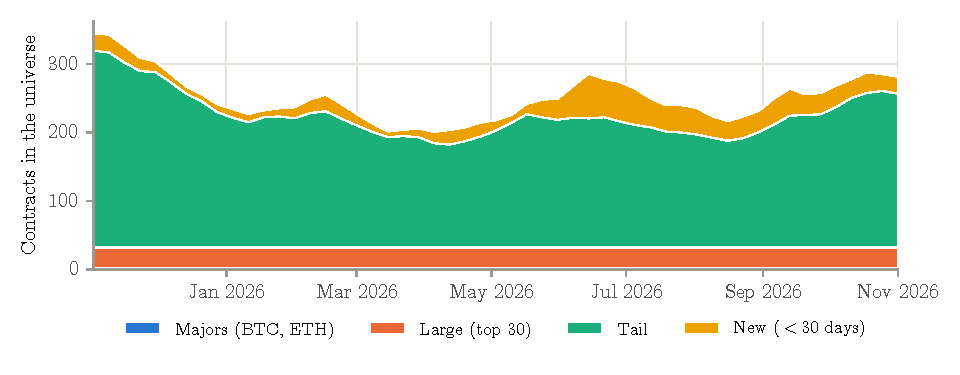
\includegraphics[width=\linewidth]{figures/fig5_universe.pdf}
\caption{Contracts in each tier, weekly mean of daily counts. The Majors tier (two contracts) is a
hairline at the bottom. New listings peaked in June and July 2026.}
\label{fig:universe}
\end{figure}

\begin{table}[t]
\centering
\caption{Data and universe, 1 November 2025 to 31 October 2026.}
\label{tab:data}
\small
\begin{tabular}{@{}lr@{}}
\toprule
Item & Value \\
\midrule
USDT-margined perpetuals in the archive (delisted included) & 924 \\
\quad with a listing date & 923 \\
\quad with 1-minute mark-price data in the study period & 900 \\
\quad in the point-in-time universe on at least one day & 753 \\
\quad of which delisted during the study & 42 \\
Balanced cohort (live for the whole study) & 424 \\
Mean contracts per day: majors / large / tail / new & 2 / 30 / 192 / 26 \\
Holding windows (1 h / 4 h / 8 h / 24 h), millions & 2.15 / 2.15 / 2.15 / 2.14 \\
\bottomrule
\end{tabular}

\end{table}

\section{Measurement}
\label{sec:measure}

\subsection{Holding windows}

Every hour, for every contract in the universe, we open a hypothetical long and a hypothetical short
at the mark price and hold each for $h\in\{1,4,8,24\}$ hours. For each window we record the return at
the end of the window and the most adverse point along it, from the minute highs and lows. A window
with any missing minute is discarded, never filled: a gap is precisely where an unobserved extreme
could lie.

\subsection{Liquidation level}
\label{sec:liq}

Consider isolated margin and a position of $Q$ contracts opened at mark price $M_0$, so that its
entry notional is $N=QM_0$ and, at leverage $L$, its initial margin is $N/L$. (On Binance's USDT
perpetuals one contract is one unit of the base asset.) A perpetual is delta-one, so profit and loss
is linear in the relative price move $x=M/M_0-1$: $+Nx$ for a long and $-Nx$ for a short.\footnote{We
refer throughout to linear (USDT- or USDC-margined) perpetuals, whose profit and loss is linear in the
price. Inverse, coin-margined perpetuals, such as Binance's COIN-M contracts or Deribit's
BTC-PERPETUAL, settle profit and loss in the base asset, $N(1-M_0/M)$ for a long, which is not linear
in the price; their liquidation level differs and is not studied here.} Liquidation occurs when
equity falls to the maintenance margin.

\paragraph{Binance's maintenance margin.} Binance computes the maintenance margin of a USDT-margined
position as
\begin{equation}
\mathrm{MM} = m_k \cdot Q \cdot M - A_k,
\end{equation}
where $Q\cdot M$ is the position notional at the current \emph{mark} price $M$ (not the index or the
last traded price), $m_k$ is the maintenance-margin rate of the notional bracket $k$ the position falls
in, and $A_k$ is that bracket's maintenance amount, which keeps the requirement continuous from one
bracket to the next~\cite{binance-margin,binance-liqprice}. A position is liquidated when the mark
price reaches its liquidation price~\cite{binance-liq}. In the first bracket $A_1=0$ for every
contract in the bracket table~\cite{binance-brackets}, so $\mathrm{MM}=m\,QM=mN(1+x)$ and
\begin{align}
\text{long:}\quad & \tfrac{1}{L} + x = m(1+x) &&\Longrightarrow\quad d_\ell = \frac{1/L - m}{1-m},\\
\text{short:}\quad & \tfrac{1}{L} - x = m(1+x) &&\Longrightarrow\quad d_s = \frac{1/L - m}{1+m}.
\end{align}
To first order the liquidation level is $1/L-m$ from entry, which is why a 50x long on BTC
($m=0.4\%$) is liquidated after 1.6\%, not 2\%. A position is admissible only if $1/L>m$. The first
bracket covers notionals up to a cap (300{,}000 USDT for BTCUSDT); larger positions face higher rates
and lower maximum leverage, so the levels studied here are those of positions within the first
bracket. Because the requirement is set on the current mark notional, it moves with the price at
rate $m$. For a long, a fall of $x$ lowers equity by $Nx$ and the requirement by $mNx$, so the gap
between them closes at rate $1-m$; for a short, a rise of $x$ lowers equity by $Nx$ and raises the
requirement by $mNx$, so the gap closes at rate $1+m$. The long therefore reaches its liquidation level
slightly later than the short: for BTC at 50x ($m=0.4\%$), after 1.606\% against 1.594\%; at 10x
with $m=2\%$, after 8.16\% against 7.84\%. Were the requirement fixed at entry, $mN$, both sides would
be liquidated at $1/L-m$.

\paragraph{Other venues.} Maintenance-margin rules differ between exchanges, in the rates and
brackets, in the price that sets the notional, and in what the requirement includes. Hyperliquid sets
the maintenance margin at half the initial margin at a contract's maximum leverage~\cite{hl-margin};
OKX adds the liquidation fee to the maintenance requirement when it computes its margin
ratio~\cite{okx-margin}. Where maintenance is set on the entry notional, $d=1/L-m$ for both sides, and
the long--short asymmetry above disappears; where collateral is held in the traded coin, as with
inverse contracts, equity itself moves with the price and the level is different again. The
liquidation levels in this paper are therefore Binance's. The unseen share, however, depends on the
level only weakly (Section~\ref{sec:results}), so the main result does not rest on any one venue's
margin rule.

\paragraph{Contract terms.} Each contract uses its own first-bracket maintenance-margin rate and
maximum leverage from Binance's bracket table, retrieved on 22 November 2026~\cite{binance-brackets}.
A leverage level that a contract does not offer is not studied for that contract. The rates range
from \MMRBTC{} for BTC and ETH to \MMRMax{}, with a median of \MMRMedian{}; a higher rate comes with
a lower maximum leverage (Table~\ref{tab:liq}). Contracts
absent from the table (\FallbackN{} in the study) take the median terms of their tier. Binance
revises brackets over time and does not publish their history, so applying current terms to the whole
year is an approximation. Fees, funding and liquidation penalties are ignored.

\subsection{\iftechnical Estimators and inference\else Aggregation and uncertainty\fi}

\iftechnical
Let $\mathcal{D}$ be the set of days, $\mathcal{S}_t$ the contracts in a tier on day $t$, and
$W_{i,t}$ the windows of contract $i$ that start on day $t$. The close-breach probability is
estimated by
\begin{equation}
\hat p_C=\frac{1}{|\mathcal D|}\sum_{t\in\mathcal D}\frac{1}{|\mathcal S_t|}\sum_{i\in\mathcal S_t}
\frac{1}{|W_{i,t}|}\sum_{w\in W_{i,t}}\1\big\{X_h^{(w)}\le -b_i\big\},
\end{equation}
and $\hat p_P$ analogously, so that each contract counts once within a day and each day counts once in
the year; $\hat U=1-\hat p_C/\hat p_P$. Quantiles use the same weights.
\else
Breach rates are computed for each contract and day, averaged across the contracts in a tier on that
day, and then averaged across days, so that each contract counts once within a day and each day counts
once in the year. A month with many new listings therefore does not dominate the result.
\fi
Windows are not independent: hourly windows overlap, and market-wide moves affect all contracts at
once. Confidence intervals therefore come from a block bootstrap that resamples whole days in blocks
of seven, preserving both dependencies. The effective sample size is the number of days, 364, rather
than the 8.6 million windows. The full measurement chain was validated on simulated random walks,
where it reproduces the theoretical benchmark to within a few percent.

\section{Results}
\label{sec:results}

\subsection{About half of all liquidations are unseen at the close}

Table~\ref{tab:breach} reports, at 10x leverage, how often the close and the path cross the
liquidation level, and the unseen share. Outside the Majors tier, between
\textbf{\UTenLo\% and \UTenHi\%} of liquidations are unseen at the close, in every tier, at every
horizon and on both sides. The difference is large in absolute terms: a 10x long in the Tail tier
held for 24 hours ends beyond its liquidation level in \TailDayLongPC{} of windows, but is liquidated
in \TailDayLongPP; for a short, the figures are \TailDayShortPC{} and \TailDayShortPP.

\begin{table}[t]
\centering
\caption{Breach probabilities at 10x leverage, mark price. $p_C$: close breach; $p_P$: path breach
(liquidation); $U=1-p_C/p_P$: unseen share, with a 95\% block-bootstrap interval. ``--'': no close
breach in the sample.}
\label{tab:breach}
\footnotesize
\setlength{\tabcolsep}{4.2pt}
\begin{tabular}{@{}llrrlrrl@{}}
\toprule
 & & \multicolumn{3}{c}{Long, 10x} & \multicolumn{3}{c}{Short, 10x} \\
\cmidrule(lr){3-5}\cmidrule(lr){6-8}
Tier & $h$ & $p_C$ & $p_P$ & $U$ [95\% CI] & $p_C$ & $p_P$ & $U$ [95\% CI] \\
\midrule
Majors & 1 h & 0.00\% & 0.00\% & -- & 0.00\% & 0.00\% & -- \\
 & 8 h & 0.02\% & 0.14\% & 88\% \scriptsize[76\%, 100\%] & 0.02\% & 0.08\% & 79\% \scriptsize[77\%, 100\%] \\
 & 24 h & 0.33\% & 1.08\% & 70\% \scriptsize[57\%, 78\%] & 0.38\% & 0.86\% & 56\% \scriptsize[40\%, 77\%] \\
\addlinespace[2pt]
Large & 1 h & 0.13\% & 0.28\% & 51\% \scriptsize[46\%, 56\%] & 0.14\% & 0.32\% & 55\% \scriptsize[51\%, 58\%] \\
 & 8 h & 1.30\% & 2.88\% & 55\% \scriptsize[51\%, 58\%] & 1.53\% & 3.37\% & 55\% \scriptsize[53\%, 57\%] \\
 & 24 h & 4.37\% & 8.96\% & 51\% \scriptsize[49\%, 54\%] & 4.31\% & 9.54\% & 55\% \scriptsize[52\%, 57\%] \\
\addlinespace[2pt]
Tail & 1 h & 0.13\% & 0.29\% & 55\% \scriptsize[51\%, 59\%] & 0.18\% & 0.37\% & 53\% \scriptsize[51\%, 54\%] \\
 & 8 h & 1.43\% & 3.15\% & 55\% \scriptsize[52\%, 57\%] & 1.99\% & 4.61\% & 57\% \scriptsize[56\%, 58\%] \\
 & 24 h & 5.00\% & 10.59\% & 53\% \scriptsize[51\%, 54\%] & 5.50\% & 13.39\% & 59\% \scriptsize[57\%, 61\%] \\
\addlinespace[2pt]
New & 1 h & 0.31\% & 0.65\% & 52\% \scriptsize[46\%, 58\%] & 0.42\% & 0.90\% & 53\% \scriptsize[50\%, 56\%] \\
 & 8 h & 3.35\% & 6.60\% & 49\% \scriptsize[48\%, 51\%] & 3.14\% & 7.71\% & 59\% \scriptsize[57\%, 61\%] \\
 & 24 h & 9.29\% & 16.93\% & 45\% \scriptsize[43\%, 48\%] & 7.19\% & 17.55\% & 59\% \scriptsize[57\%, 61\%] \\
\bottomrule
\end{tabular}

\end{table}

Figure~\ref{fig:hidden} shows $U$ across leverage levels. It lies close to the random-walk value of
50\% almost everywhere, and a few points above it in most cells. The blind spot is therefore
\emph{structural}: a measure that looks only at the close misses about half of all liquidations even
in an idealised market\iftechnical{} (Corollary~\ref{cor:half})\fi, and crypto price paths do not
improve on that. The Majors tier stands out, at \MajorsDayU\% for a 24-hour 10x long, but on few
events and with wide intervals: BTC and ETH rarely move 10\% within a day.

\begin{figure}[t]
\centering
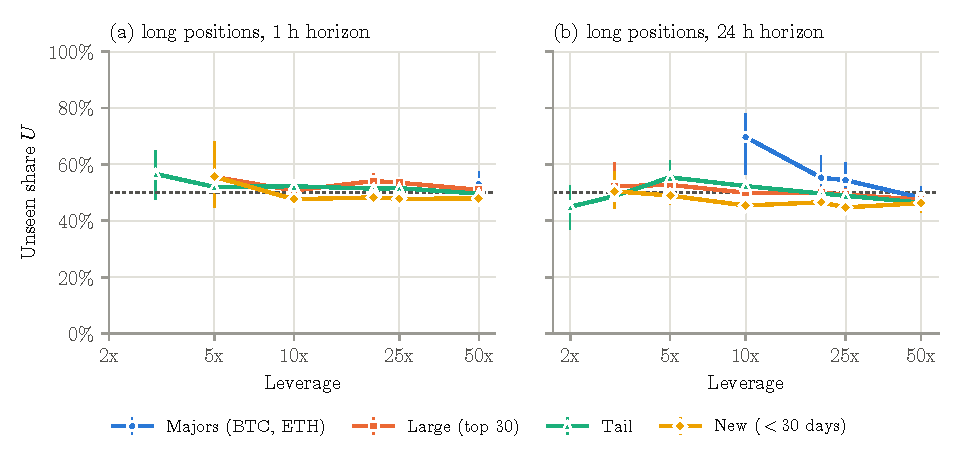
\includegraphics[width=\linewidth]{figures/fig2_hidden_share.pdf}
\caption{Unseen share $U$ for long positions, mark price, with 95\% block-bootstrap intervals. Points
whose interval is wider than 25 percentage points (too few close breaches) are omitted, which removes
most low-leverage Majors points. Dotted line: random-walk benchmark, 50\%.}
\label{fig:hidden}
\end{figure}

\subsection{At 10x, 25x and 50x}

Table~\ref{tab:leverage} sets the three leverage levels side by side for long positions, together
with the share of each tier's windows in which the contract offers that leverage. As leverage rises,
both breach probabilities rise steeply while $U$ stays near one half, so the \emph{number} of
liquidations a close-to-close view misses grows with leverage. For a long held one hour in the Tail
tier, the liquidation probability is \TailHourPPTen{} at 10x, \TailHourPPTwentyFive{} at 25x and
\TailHourPPFifty{} at 50x, against close-breach probabilities of \TailHourPCTen, \TailHourPCTwentyFive{}
and \TailHourPCFifty. Held for 24 hours, a 50x long in the Tail tier is liquidated in \TailDayPPFifty{}
of windows, while only \TailDayPCFifty{} end beyond the level; at 25x in the Large tier the figures
are \LargeDayPPTwentyFive{} and \LargeDayPCTwentyFive. Outside the Majors tier, the unseen share stays
between \LevULo\% and \LevUHi\% in every cell of the table.

The share does not grow with leverage because it is a ratio. A closer liquidation level raises the
probability of touching it and the probability of ending beyond it together, and for a random walk
the first is twice the second at every distance\iftechnical{} (Corollary~\ref{cor:half})\fi. Higher
leverage therefore multiplies the liquidations a close-to-close view misses, while the fraction it
misses stays near one half. In the example of
Figure~\ref{fig:example}, the 50x position was closed within twelve minutes of entry.

\begin{table}[t]
\centering
\caption{Long positions at 10x, 25x and 50x, mark price, each contract with its own
maintenance-margin rate. \emph{Offered}: share of the tier's windows in which the contract offers that
leverage. $p_C$, $p_P$: close and path breach probabilities; $U$: unseen share.}
\label{tab:leverage}
\footnotesize
\begin{tabular}{@{}llrrrrrrr@{}}
\toprule
 & & & \multicolumn{3}{c}{1 h} & \multicolumn{3}{c}{24 h} \\
\cmidrule(lr){4-6}\cmidrule(lr){7-9}
Tier & $L$ & $d_{\text{long}}$ & $p_C$ & $p_P$ & $U$ & $p_C$ & $p_P$ & $U$ \\
\midrule
Majors & 10x & 9.64\% & 0.00\% & 0.00\% & -- & 0.33\% & 1.08\% & 70\% \\
 & 25x & 3.61\% & 0.07\% & 0.22\% & 68\% & 7.39\% & 16.20\% & 54\% \\
 & 50x & 1.61\% & 1.17\% & 2.50\% & 53\% & 23.33\% & 44.99\% & 48\% \\
\addlinespace[2pt]
Large & 10x & 9.55\% & 0.13\% & 0.28\% & 51\% & 4.37\% & 8.96\% & 51\% \\
 & 25x & 3.52\% & 1.20\% & 2.56\% & 53\% & 19.98\% & 39.06\% & 49\% \\
 & 50x & 1.51\% & 6.13\% & 12.62\% & 51\% & 34.96\% & 66.04\% & 47\% \\
\addlinespace[2pt]
Tail & 10x & 9.09\% & 0.13\% & 0.29\% & 55\% & 5.00\% & 10.59\% & 53\% \\
 & 25x & 3.03\% & 1.77\% & 3.63\% & 51\% & 25.59\% & 50.36\% & 49\% \\
 & 50x & 1.01\% & 13.04\% & 26.17\% & 50\% & 42.87\% & 80.35\% & 47\% \\
\addlinespace[2pt]
New & 10x & 9.09\% & 0.31\% & 0.65\% & 52\% & 9.29\% & 16.93\% & 45\% \\
 & 25x & 3.03\% & 3.60\% & 6.97\% & 48\% & 25.28\% & 47.29\% & 47\% \\
 & 50x & 1.01\% & 14.57\% & 27.90\% & 48\% & 38.70\% & 72.84\% & 47\% \\
\bottomrule
\end{tabular}

\end{table}

\subsection{The tail of the path is heavier than the tail of the close}

The unseen share measures how often. Table~\ref{tab:quantiles} and Figure~\ref{fig:quantiles}
measure how far. For every tier, horizon and side, the 99th percentile of the adverse move along the
path is \textbf{\KappaLo{} to \KappaHi{} times} the 99th percentile of the close-to-close loss,
against $1.107$ for a random walk\iftechnical{} (Proposition~\ref{prop:kappa})\fi. For a one-hour
long in the Large tier, the close-to-close 1-in-100 loss is \LargeHourQC; the path reaches
\LargeHourQP.

\begin{table}[t]
\centering
\caption{99th-percentile adverse move at the close ($Q^C_{0.99}$) and along the path ($Q^P_{0.99}$),
mark price, and their ratio $\kappa_{0.99}$. Weighted so that each day, and each contract within a
day, counts once. These do not depend on leverage.}
\label{tab:quantiles}
\footnotesize
\begin{tabular}{@{}llrrrrrr@{}}
\toprule
 & & \multicolumn{3}{c}{1 h} & \multicolumn{3}{c}{24 h} \\
\cmidrule(lr){3-5}\cmidrule(lr){6-8}
Tier & Side & $Q_{0.99}^{C}$ & $Q_{0.99}^{P}$ & $\kappa_{0.99}$ & $Q_{0.99}^{C}$ & $Q_{0.99}^{P}$ & $\kappa_{0.99}$ \\
\midrule
Majors & Long & 1.71\% & 2.26\% & 1.32 & 7.29\% & 9.88\% & 1.36 \\
 & Short & 1.60\% & 2.11\% & 1.32 & 7.74\% & 9.31\% & 1.20 \\
\addlinespace[2pt]
Large & Long & 3.81\% & 5.38\% & 1.41 & 18.95\% & 26.16\% & 1.38 \\
 & Short & 4.02\% & 5.67\% & 1.41 & 21.13\% & 31.67\% & 1.50 \\
\addlinespace[2pt]
Tail & Long & 3.90\% & 5.34\% & 1.37 & 17.04\% & 23.04\% & 1.35 \\
 & Short & 4.20\% & 5.84\% & 1.39 & 22.77\% & 35.65\% & 1.57 \\
\addlinespace[2pt]
New & Long & 5.74\% & 7.72\% & 1.35 & 23.82\% & 28.84\% & 1.21 \\
 & Short & 5.94\% & 8.48\% & 1.43 & 30.38\% & 49.55\% & 1.63 \\
\addlinespace[2pt]
\multicolumn{2}{@{}l}{Brownian benchmark} & & & 1.107 & & & 1.107 \\
\bottomrule
\end{tabular}

\end{table}

\begin{figure}[t]
\centering
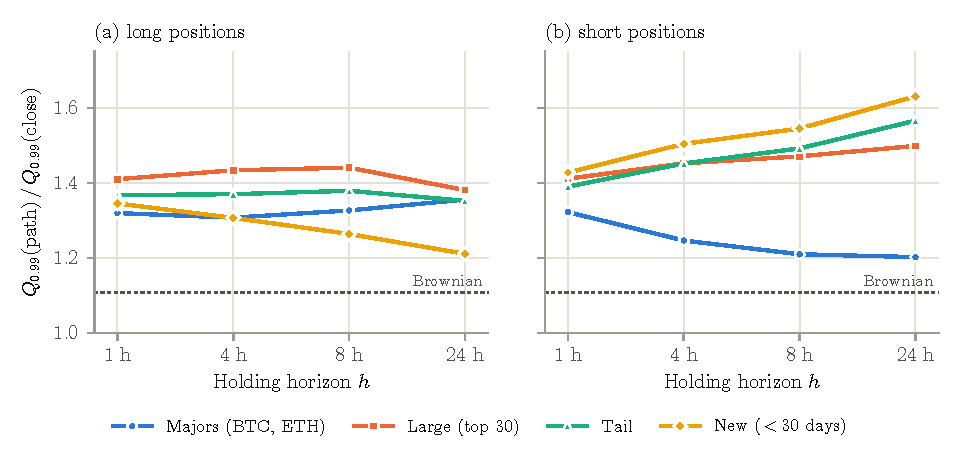
\includegraphics[width=\linewidth]{figures/fig3_quantile_multiple.pdf}
\caption{Path-to-close quantile multiple $\kappa_{0.99}$ by holding horizon. Dotted line: random-walk
benchmark, $1.107$.}
\label{fig:quantiles}
\end{figure}

\subsection{Short positions and new listings}

The two sides behave differently. For longs, $\kappa_{0.99}$ is roughly constant across horizons.
For shorts outside the Majors tier, it rises with the horizon, from about 1.4 at one hour to 1.5--1.6
at 24 hours, and is highest for new listings, at \KappaHi. Upward spikes that subsequently fade,
typical of squeezes in thin and newly listed contracts, liquidate short positions without leaving a
trace in the closing price.

\section{Robustness}
\label{sec:robust}

\paragraph{Survivorship.} We repeat the analysis on a balanced cohort: the 424 contracts that were
past their 30-day burn-in on 1 November 2025 and still trading on 31 October 2026. The cohort is
biased towards survivors and should therefore \emph{understate} path risk. The results change little
(Table~\ref{tab:robust}): quantile multiples move by at most \CohortMaxDK, and unseen shares by at
most \CohortMaxDU{} percentage points. The findings are not an artefact of the changing universe.

\paragraph{Mark price versus traded price.} All results use the mark price, on which liquidation is
triggered. The mark price is a smoothed construction; on Binance it is a median of index-based
estimates and the contract price~\cite{binance-mark}. Measured on last traded prices instead,
close-to-close risk is almost unchanged but path risk rises: for a 10x long held one hour, $U$ moves
from \RobLargeMark\% to \RobLargeLast\% in the Large tier and from \RobTailMark\% to \RobTailLast\% in
the Tail tier (Figure~\ref{fig:marklast}). The smoothing removes some short-lived wicks. The
mark-price figures are therefore a conservative description of the price path a trader sees on the
chart; the smoothing does not remove the effect.

\begin{table}[t]
\centering
\caption{Robustness. \emph{Mark}: main study. \emph{Cohort}: mark price, the 424 contracts live for
the whole period (no New tier by construction). \emph{Last}: same universe, last traded prices. ``--'':
no close breach.}
\label{tab:robust}
\footnotesize
\setlength{\tabcolsep}{4.5pt}
\begin{tabular}{@{}lrrrrrrrrr@{}}
\toprule
 & \multicolumn{3}{c}{$\kappa_{0.99}$, long, 1 h} & \multicolumn{3}{c}{$U$, 10x long, 1 h} & \multicolumn{3}{c}{$\kappa_{0.99}$, short, 24 h} \\
\cmidrule(lr){2-4}\cmidrule(lr){5-7}\cmidrule(lr){8-10}
Tier & Mark & Cohort & Last & Mark & Cohort & Last & Mark & Cohort & Last \\
\midrule
Majors & 1.32 & 1.32 & 1.35 & -- & -- & -- & 1.20 & 1.20 & 1.22 \\
Large & 1.41 & 1.41 & 1.51 & 51\% & 57\% & 59\% & 1.50 & 1.45 & 1.53 \\
Tail & 1.37 & 1.37 & 1.47 & 55\% & 57\% & 63\% & 1.57 & 1.60 & 1.60 \\
New & 1.35 & -- & 1.43 & 52\% & -- & 59\% & 1.63 & -- & 1.66 \\
\bottomrule
\end{tabular}

\end{table}

\begin{figure}[t]
\centering
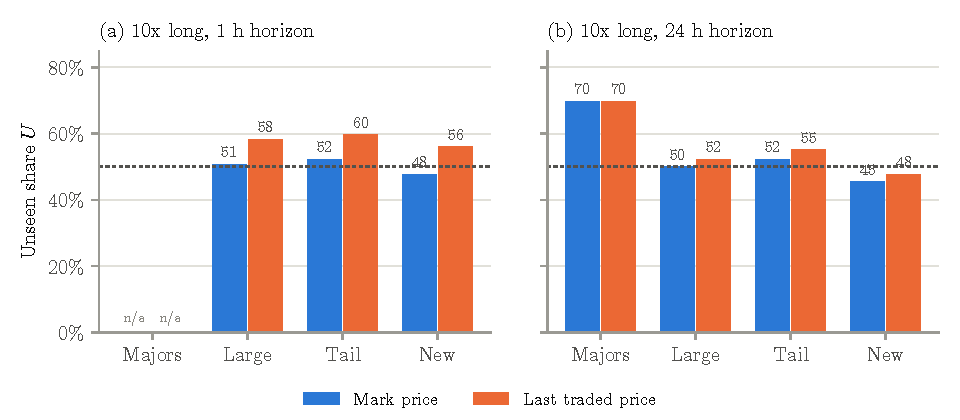
\includegraphics[width=\linewidth]{figures/fig4_mark_vs_last.pdf}
\caption{Unseen share $U$ for a 10x long, measured on the mark price and on the last traded price.
Dotted line: random-walk benchmark. Majors at one hour: no close breach.}
\label{fig:marklast}
\end{figure}

\section{Implications for risk measurement}

\begin{enumerate}\itemsep2pt
\item \textbf{Measure the path, not the close.} Value-at-risk and volatility for leveraged positions
should be estimated from the most adverse point of the price over the holding period, or from
range-based estimators~\cite{parkinson,garmanklass,rogerssatchell}, not from closing returns alone.
\item \textbf{Match the horizon to the monitoring.} Liquidation is checked continuously. A daily risk
figure describes the end of the day; the position must survive every moment before it.
\item \textbf{Scale closing-price tails up, asymmetrically.} Where only close-to-close statistics
are available, these data indicate that the 1-in-100 adverse move along the path is 20--45\% larger
than the closing loss for longs, and up to 63\% larger for shorts in thin or newly listed contracts.
\item \textbf{Treat new listings as a separate regime.} The first 30 days carry the highest
close-to-close risk and the heaviest path tail for short positions.
\end{enumerate}

\section{Limitations}

Maintenance-margin rates and maximum leverage are each contract's current first bracket, applied to
the whole year, because Binance does not publish their history; larger positions fall into higher
brackets with higher rates and lower leverage. Fees, funding and liquidation penalties are ignored.
Positions use isolated margin; cross margin pools collateral and changes the level. The study covers
one venue and one year. The liquidity threshold (\$5 million a day) and the 30-day burn-in are design
choices; the balanced-cohort check suggests that the conclusions do not depend on the composition of
the universe.

\section{Conclusion}
\label{sec:conclusion}

Crypto perpetual futures trade around the clock and liquidate at the first touch of the liquidation
level, at leverage of up to 150x on the largest venues and 20--25x on the median contract. In that
setting, the close-to-close return is the wrong object for measuring risk. Half of all liquidations
are invisible at the close even in an idealised random market, and on a full year of Binance data,
with each contract's own margin terms and delisted contracts included, the share is between
\UTenLo\% and \UTenHi\% at 10x and between \UTwentyFiveLo\% and \UTwentyFiveHi\% at 25x outside BTC
and ETH. The share is stable; the count is not. A day-long 25x long in the Tail tier is liquidated in
\TailDayLongPPTwentyFive{} of windows, against \TailDayLongPP{} at 10x. The tail is worse than the frequency suggests: the 1-in-100 adverse move along the path is
\KappaLo{} to \KappaHi{} times the close-to-close figure, well above the random-walk value of 1.107,
and worst for short positions in newly listed contracts. Neither result depends on survivorship, and
neither is an artefact of mark-price smoothing.

The practical conclusion is a warning. Volatility, value-at-risk and leverage limits estimated from
closing prices, daily or otherwise, systematically understate the risk of leveraged positions on 24/7
crypto venues, for traders sizing positions and for platforms and risk managers setting margin
alike. Risk measured for these markets should be measured on the path, at the frequency at which
liquidation is monitored.

\paragraph{Code and data.} All results are computed from public data by an open pipeline, from
download to the figures and tables in this paper, together with both editions of the paper:
\url{https://github.com/PTR-25/crypto-path-risk}.

\begin{thebibliography}{99}\small\raggedright
\bibitem{binance-liq} Binance. Binance Futures liquidation protocols. Help centre,
\url{https://www.binance.com/en/support/faq/360033525271}, accessed 22 November 2026.
\bibitem{binance-margin} Binance. Leverage and margin of USDS-M
futures. Help centre, \url{https://www.binance.com/en/support/faq/360033162192}, accessed 22 November
2026.
\bibitem{binance-liqprice} Binance. How to calculate liquidation price of USDS-M
futures contracts. Help centre,
\url{https://www.binance.com/en/support/faq/b3c689c1f50a44cabb3a84e663b81d93}, accessed 22 November
2026.
\bibitem{binance-mark} Binance. What are mark price and price index in USD-margined futures? Help
centre, \url{https://www.binance.com/en/support/faq/360033525071}, accessed 22 November 2026.
\bibitem{binance-brackets} Binance. Futures leverage and margin brackets, public feed of the Leverage
\& Margin page, \url{https://www.binance.com/bapi/futures/v1/friendly/future/common/brackets},
retrieved 22 November 2026.
\bibitem{bybit-mark} Bybit. Mark price calculation (perpetual contracts). Help centre,
\url{https://www.bybit.com/en/help-center/article/Mark-Price-Calculation-Perpetual-Contracts},
accessed 22 November 2026.
\bibitem{bybit-api} Bybit. V5 API, instruments info,
\url{https://api.bybit.com/v5/market/instruments-info?category=linear}, retrieved 22 November 2026.
\bibitem{okx-liq} OKX. System liquidation mechanism. Help centre,
\url{https://www.okx.com/en-us/help/system-liquidation-mechanism-eea}, accessed 22 November 2026.
\bibitem{okx-margin} OKX. Futures margin calculation rules. Help centre,
\url{https://www.okx.com/en-us/help/futures-margin-calculation-rules}, accessed 22 November 2026.
\bibitem{okx-api} OKX. V5 API, public instruments,
\url{https://www.okx.com/api/v5/public/instruments?instType=SWAP}, retrieved 22 November 2026.
\bibitem{deribit-api} Deribit. API v2, public/get\_instruments,
\url{https://www.deribit.com/api/v2/public/get_instruments?currency=USDC&kind=future}, retrieved 22
November 2026.
\bibitem{hl-margin} Hyperliquid. Margining. Documentation,
\url{https://hyperliquid.gitbook.io/hyperliquid-docs/trading/margining}, accessed 22 November 2026.
\bibitem{hl-liq} Hyperliquid. Liquidations. Documentation,
\url{https://hyperliquid.gitbook.io/hyperliquid-docs/trading/liquidations}, accessed 22 November 2026.
\bibitem{hl-api} Hyperliquid. Info endpoint, perpetuals metadata, \url{https://api.hyperliquid.xyz/info},
retrieved 22 November 2026.
\bibitem{bgk} M.~Broadie, P.~Glasserman and S.~Kou. A continuity correction for discrete barrier
options. \emph{Mathematical Finance} 7(4), 325--349, 1997.
\bibitem{garmanklass} M.~B.~Garman and M.~J.~Klass. On the estimation of security price
volatilities from historical data. \emph{Journal of Business} 53(1), 67--78, 1980.
\bibitem{parkinson} M.~Parkinson. The extreme value method for estimating the variance of the rate of
return. \emph{Journal of Business} 53(1), 61--65, 1980.
\bibitem{rogerssatchell} L.~C.~G.~Rogers and S.~E.~Satchell. Estimating variance from high, low and
closing prices. \emph{Annals of Applied Probability} 1(4), 504--512, 1991.
\end{thebibliography}

\appendix
\section{Binance maintenance-margin rates and liquidation levels}

\begin{table}[H]
\centering
\caption{Binance USDT perpetuals by first-bracket maintenance-margin rate $m$, retrieved 22 November
2026: number of contracts, median maximum leverage, and the adverse move to liquidation $d_\ell$ of a
long, in \%, at selected leverage. ``--'': not admissible ($1/L\le m$). Short-side levels are
$d_s=d_\ell(1-m)/(1+m)$.}
\label{tab:liq}
\footnotesize
\begin{tabular}{@{}rrrrrrrrrr@{}}
\toprule
$m$ & Contracts & Max lev. & 10x & 20x & 25x & 50x & 75x & 100x & 150x \\
\midrule
0.40\% & 2 & 150x & 9.64 & 4.62 & 3.61 & 1.61 & 0.94 & 0.60 & 0.27 \\
0.50\% & 18 & 100x & 9.55 & 4.52 & 3.52 & 1.51 & 0.84 & 0.50 & 0.17 \\
0.60\% & 10 & 75x & 9.46 & 4.43 & 3.42 & 1.41 & 0.74 & 0.40 & 0.07 \\
0.65\% & 8 & 75x & 9.41 & 4.38 & 3.37 & 1.36 & 0.69 & 0.35 & 0.02 \\
1.00\% & 136 & 75x & 9.09 & 4.04 & 3.03 & 1.01 & 0.34 & -- & -- \\
1.20\% & 2 & 35x & 8.91 & 3.85 & 2.83 & 0.81 & 0.13 & -- & -- \\
1.50\% & 193 & 50x & 8.63 & 3.55 & 2.54 & 0.51 & -- & -- & -- \\
2.00\% & 131 & 25x & 8.16 & 3.06 & 2.04 & -- & -- & -- & -- \\
2.50\% & 229 & 20x & 7.69 & 2.56 & 1.54 & -- & -- & -- & -- \\
3.00\% & 12 & 20x & 7.22 & 2.06 & 1.03 & -- & -- & -- & -- \\
4.00\% & 7 & 20x & 6.25 & 1.04 & -- & -- & -- & -- & -- \\
5.00\% & 160 & 10x & 5.26 & -- & -- & -- & -- & -- & -- \\
8.00\% & 2 & 8x & 2.17 & -- & -- & -- & -- & -- & -- \\
10.00\% & 17 & 5x & -- & -- & -- & -- & -- & -- & -- \\
\bottomrule
\end{tabular}

\end{table}

\end{document}
